An \textit{n}-body simulation is a simulation of \textit{n} bodies, as the name
would suggest. We simulate the interactions of these \textit{n} bodies. The
bodies are located in a three-dimensional space. In each tick the simulation
calculates the every points interaction, with all the other points. The
interaction can vary, with gravitational attraction being the simplest.

If we were to compute the interaction for each body at
each tick, naively, we would have a running time of $O(n^2)$, and since the
simulation could be expected to work on very large values of $n$, as well as the
interaction
might be timeconsuming to calculate, it will end up being very slow. Therefore we
implement a clustered version instead. The idea is that by defining clusters of
bodies we can approximate a region of points, as a single point. The clustered
version is tree-based meaning that we store the points in a tree, and based on
some threshold $\theta$ we determine when we should calculate the interaction
for actual points, and when to calculate it for th clustered representation.
\subsection{Barnes-Hut simulation}
To perform this clustered \textit{n}-body simulation, we make use of the
Barnes-Hut algorithm \cite{BH-algo}. In Barnes-Hut an octree for 3D, or a
quadtree for 2D, is typically used. This is typically done since the space
containing these bodies can be subdivided into these types of trees. An exmaple
of this can be seen in figure \ref{fig:subdivision}.
\begin{Figure}
  \centering
  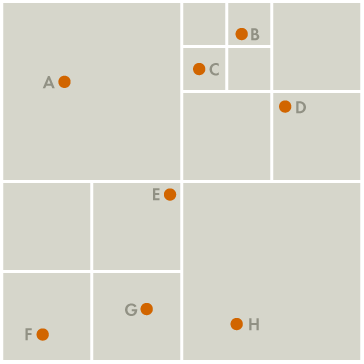
\includegraphics[width=0.30\textwidth]{assests/example-space}
  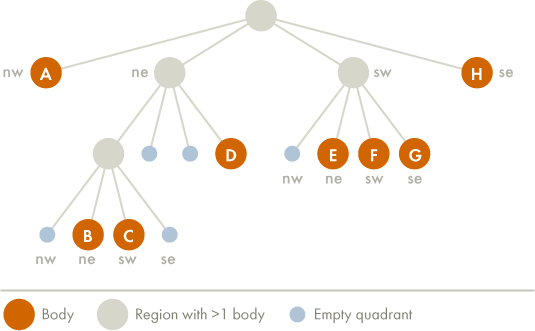
\includegraphics[width=0.65\textwidth]{assests/example-tree}
  \captionof{figure}{A sample space subdivided into regions, with each region
    containing 1 body. The quadtree created from this 2D space can also be seen.}
  \label{fig:subdivision}
\end{Figure}
